Mobile health is quickly emerging as an important topic in Computer Science. As mobile phones become increasingly powerful and prominent in everyday life, their potential to be used to improve healthcare outside of the hospital also increases. Oftentimes, an emergency response team needs access to the healthcare records of a patient in order to better provide care to that individual. To further complicate this problem, the patient's records may not be available at the hospital that the emergency response team belongs to. The patient may be traveling and his records may be at his home hospital in another area. This scenario is illustrated in Figure 1.

\begin{figure}[h]
\begin{center}
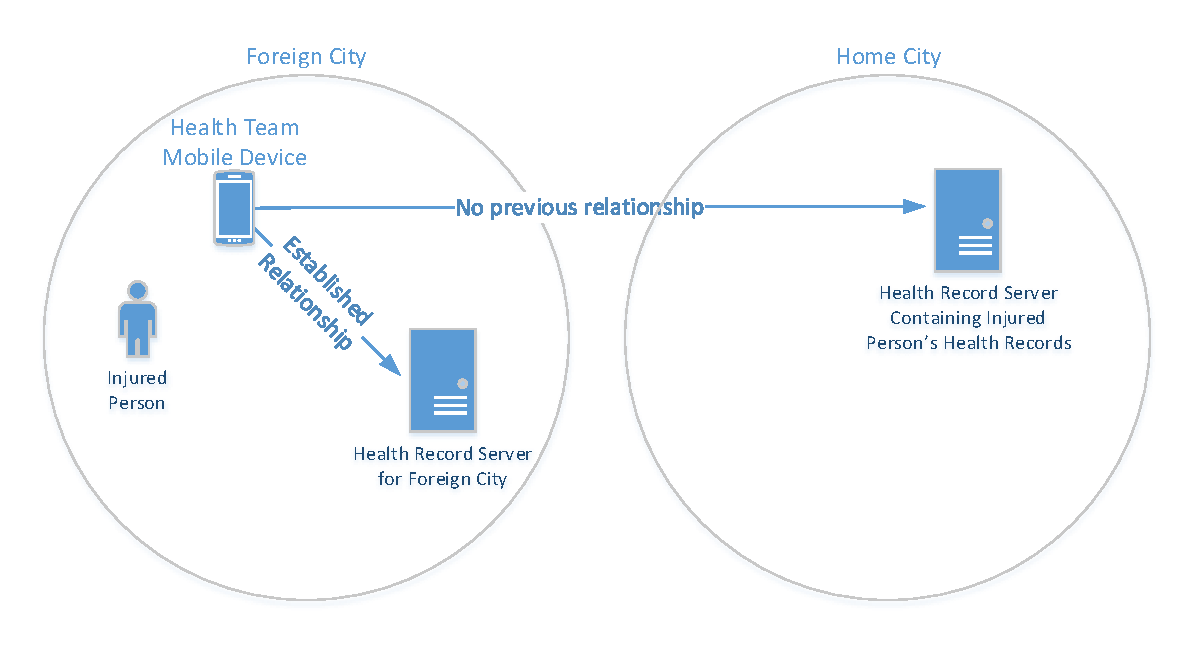
\includegraphics[scale=.75]{Drawing1.pdf}
\caption{The emergency health response team cannot access the patient's records.}
\end{center}
\end{figure}

The problem of retrieving these health records using a mobile phone does not currently have an accepted solution in use. After exploring currently proposed solutions, we attempt to combine these, as well as our own ideas, into a protocol of our creation.

In this protocol, there are two primary types of servers --- Health Record Servers and Trust Servers. Trust Servers are responsible for validating the identity of anyone that wants access to health records. These Trust Servers return an identity token which serves to confirm the trust that the Trust Servers have placed in the holder. This token can be presented to the Health Record Servers to access the needed records. The design of this protocol allows parties that may have no prior knowledge of each other to interact with some degree of trust.

Chains of trust are used utilized by the Trust Servers to deliver the identity token. A single trust server may not have the information or trust necessary to return the identity token by itself. Instead, it can contact another Trust Server that may have more ability to generate the identity token. Through this, a chain of trust is built. The first Trust Server vouches for the identity of the individual requesting the token. The second Trust Server may not know the individual, but places its trust in the first Trust Server and carries out the request. In the process of carrying out the request, the second Trust Server may have to contact additional Trust Servers, thereby lengthening the chain. This chain of trust is what allows the trusted interaction of previously unknown parties.

A prototype implementation of the protocol with several components is also constructed. The first of these components is an Android client that simulates what an emergency health care team may be using. The Android application communicates with Tomcat servers that represent several parties that interact in order to deliver the health records securely to the Android application.

This protocol was conceived after analysis of related works, which are highlighted in the following section. Section 3 discusses the design decisions and implementation process that went into the prototype. Section 4 contains conclusions drawn from the prototype development and testing, and section 5 discusses future directions for the project. Appendix A contains the code for the Android application used in the prototype, and Appendix B contains the Tomcat servlet code.